% !TEX TS-program = pdflatex
% !TEX encoding = UTF-8 Unicode

% This file is a template using the "beamer" package to create slides for a talk or presentation
% - Giving a talk on some subject.
% - The talk is between 15min and 45min long.
% - Style is ornate.

% MODIFIED by Jonathan Kew, 2008-07-06
% The header comments and encoding in this file were modified for inclusion with TeXworks.
% The content is otherwise unchanged from the original distributed with the beamer package.

\documentclass{beamer}

\mode<presentation>
{
  \usetheme{Malmoe}
  % or ...

  %\setbeamercovered{transparent}
  % or whatever (possibly just delete it)
}


\usepackage[english]{babel}
\usepackage{graphicx}
\usepackage{amssymb}
\usepackage{multicol,multirow,array}
\setbeamertemplate{navigation symbols}{}%remove navigation symbols
\setbeamertemplate{footline}[frame number]


\title[Association Testing with X Chromosome Data] % (optional, use only with long paper titles)
{Association Testing with X Chromosome Data:\\
Adding to Our Pipeline}

%\subtitle
%{Presentation Subtitle} % (optional)

\author[Caitlin McHugh, with Tim Thornton\\Adrienne Stilp\\Matt Conomos\\Cathy Laurie] % (optional, use only with lots of authors)
{Caitlin McHugh, with Tim Thornton\\Adrienne Stilp\\Matt Conomos\\Cathy Laurie}
% - Use the \inst{?} command only if the authors have different
%   affiliation.

\institute[University of Washington] % (optional, but mostly needed)
{
  Department of Biostatistics\\
  University of Washington
}
% - Use the \inst command only if there are several affiliations.
% - Keep it simple, no one is interested in your street address.

\date[Short Occasion] % (optional)
{24 August 2015}

% If you have a file called "university-logo-filename.xxx", where xxx
% is a graphic format that can be processed by latex or pdflatex,
% resp., then you can add a logo as follows:

% \pgfdeclareimage[height=0.5cm]{university-logo}{university-logo-filename}
% \logo{\pgfuseimage{university-logo}}

% If you wish to uncover everything in a step-wise fashion, uncomment
% the following command: 

%\beamerdefaultoverlayspecification{<+->}


\begin{document}

\begin{frame}
  \titlepage
\end{frame}

\begin{frame}{Outline}
 \tableofcontents
  % You might wish to add the option [pausesections]
\end{frame}

% update on adding x chr effects to the pipeline

\begin{frame}{Update on adding X chromosome effects to the pipeline}
\begin{itemize}
\item Should we adjust for random effects on the X + X chromosome PCs 1-2 when testing an autosomal SNP?
\item \textcolor{blue}{Only if X effects are confounders.}
\end{itemize}
\end{frame}

\section[]{LRT on autosomal / X chr SNPs}
\begin{frame}{Are X chromosome effects confounders?}
\begin{itemize}
\item In a set of unrelated samples, regress 
\begin{align*}
\mbox{auto genotype }&\sim \mbox{auto PC }1-5\\
\mbox{auto genotype }&\sim \mbox{auto PC }1-5 + \mbox{X chr PC }1-2
\end{align*}
\item Perform the likelihood ratio test (LRT) comparing these models.
\item Examine QQ and Manhattan plots.
\end{itemize}
\end{frame}

\begin{frame}{Results when testing auto genotypes}
\begin{figure}
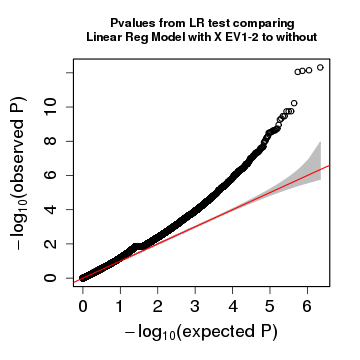
\includegraphics[height=3.8cm]{../olga_update_27july2015/qqPlot_autoSNPs.png}
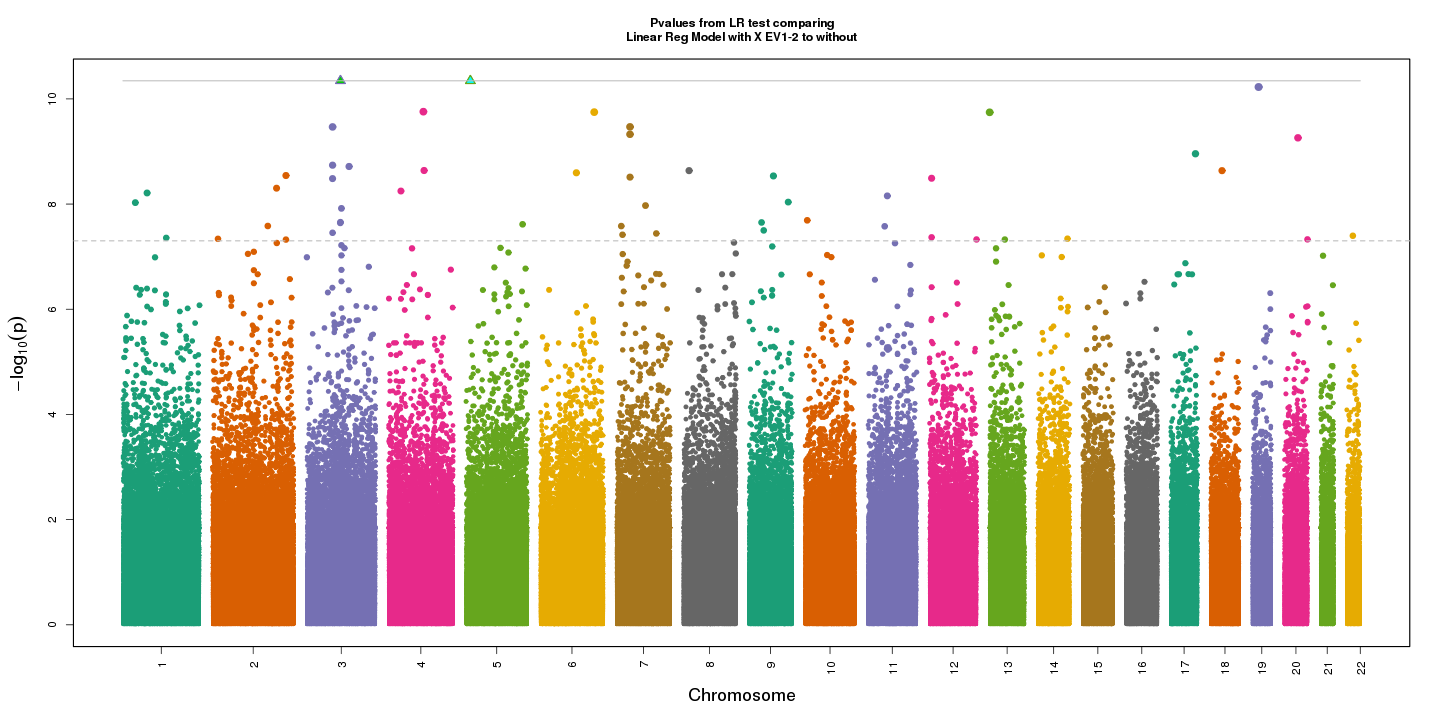
\includegraphics[width=8cm]{../olga_update_27july2015/manhPlot_autoSNPs.png}
\end{figure}
\end{frame}



\begin{frame}{Are X chromosome effects confounders?}
\begin{itemize}
\item In a set of unrelated samples, regress 
\begin{align*}
\mbox{X genotype }&\sim \mbox{X chr PC }1-2\\
\mbox{X genotype }&\sim \mbox{X chr PC }1-2 + \mbox{auto PC }1-5
\end{align*}
\item Perform LRT comparing these models.
\item Examine QQ and Manhattan plots.
\end{itemize}
\end{frame}


\begin{frame}{Results when testing X chromosome genotypes}
\begin{figure}
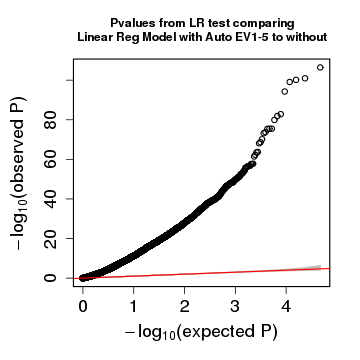
\includegraphics[height=3.8cm]{../olga_update_27july2015/qqPlot_xSNPs.png}
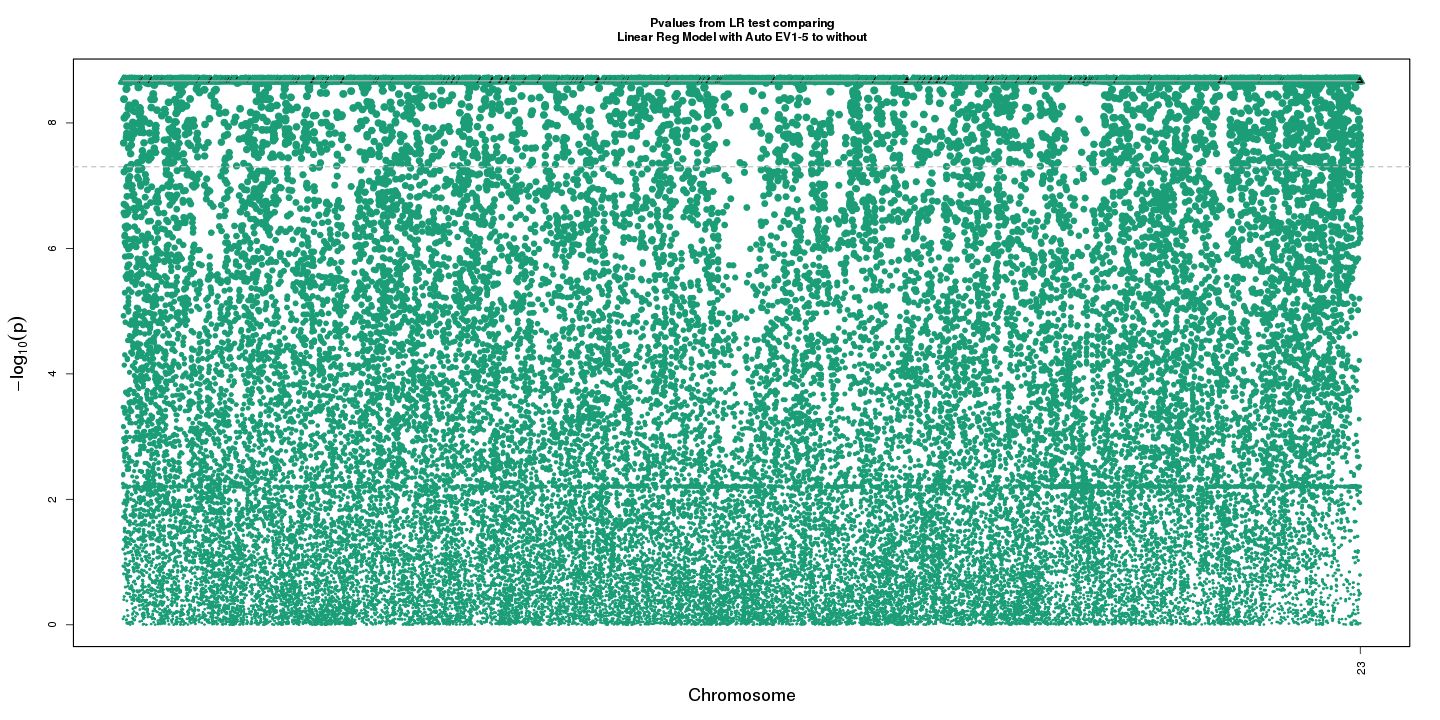
\includegraphics[width=8cm]{../olga_update_27july2015/manhPlot_xSNPs.png}
\end{figure}
\end{frame}


\section[]{More results with X KC}
\begin{frame}{Recall: on the X}
X chromosome KC for autosomally unrelated samples.
\begin{figure}
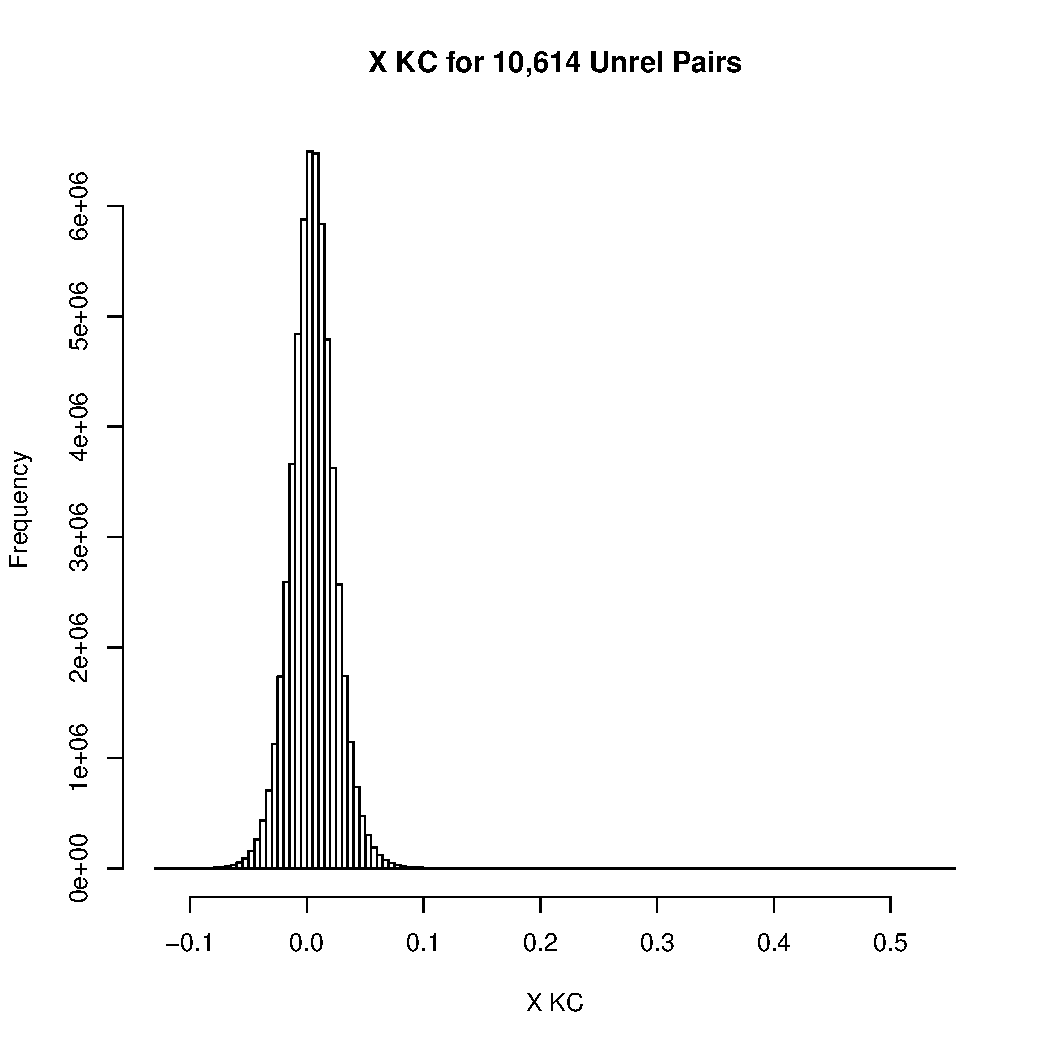
\includegraphics[height=6cm]{../xkc_unrel_hist.pdf}
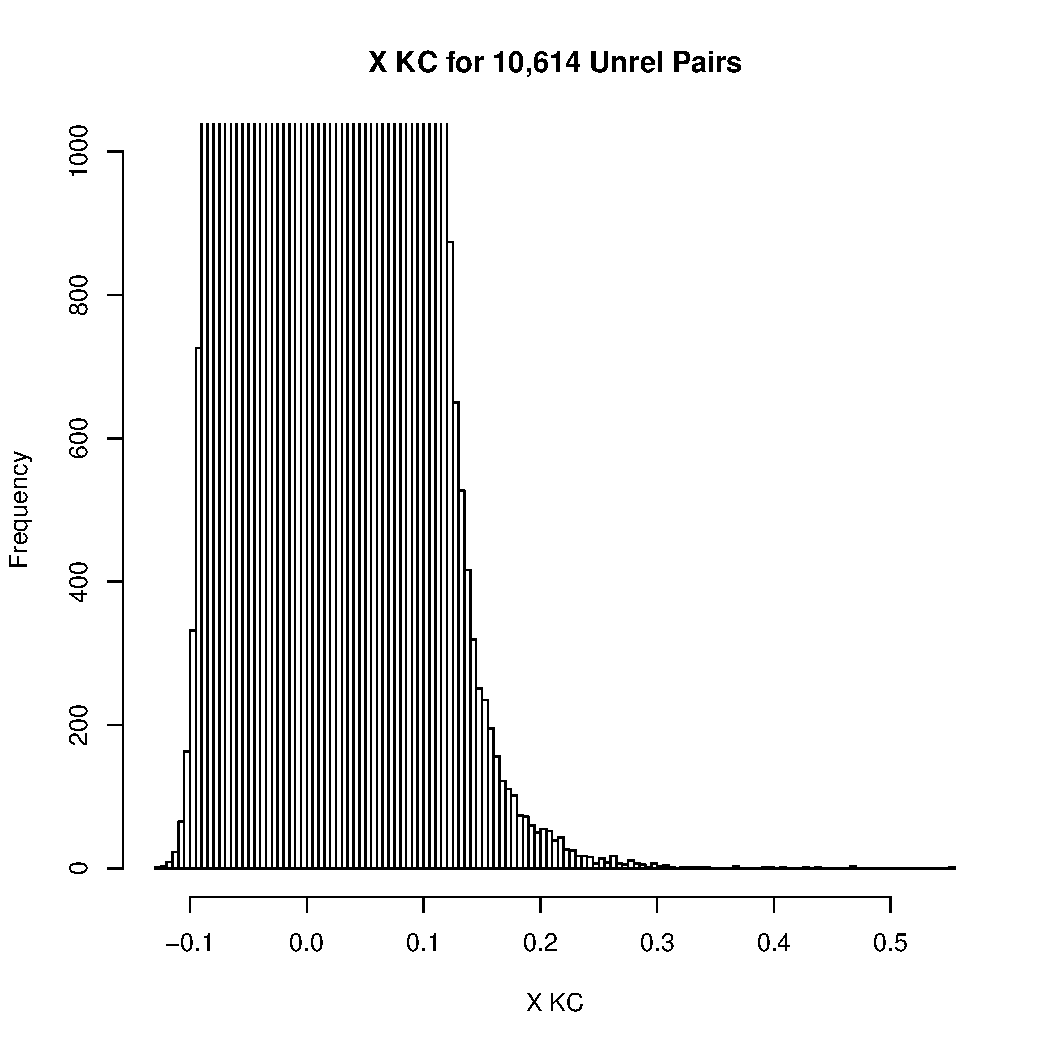
\includegraphics[height=6cm]{../xkc_unrel_hist_trunc.pdf}
\end{figure}
\end{frame}

\begin{frame}{X KC by sex}
\begin{figure}
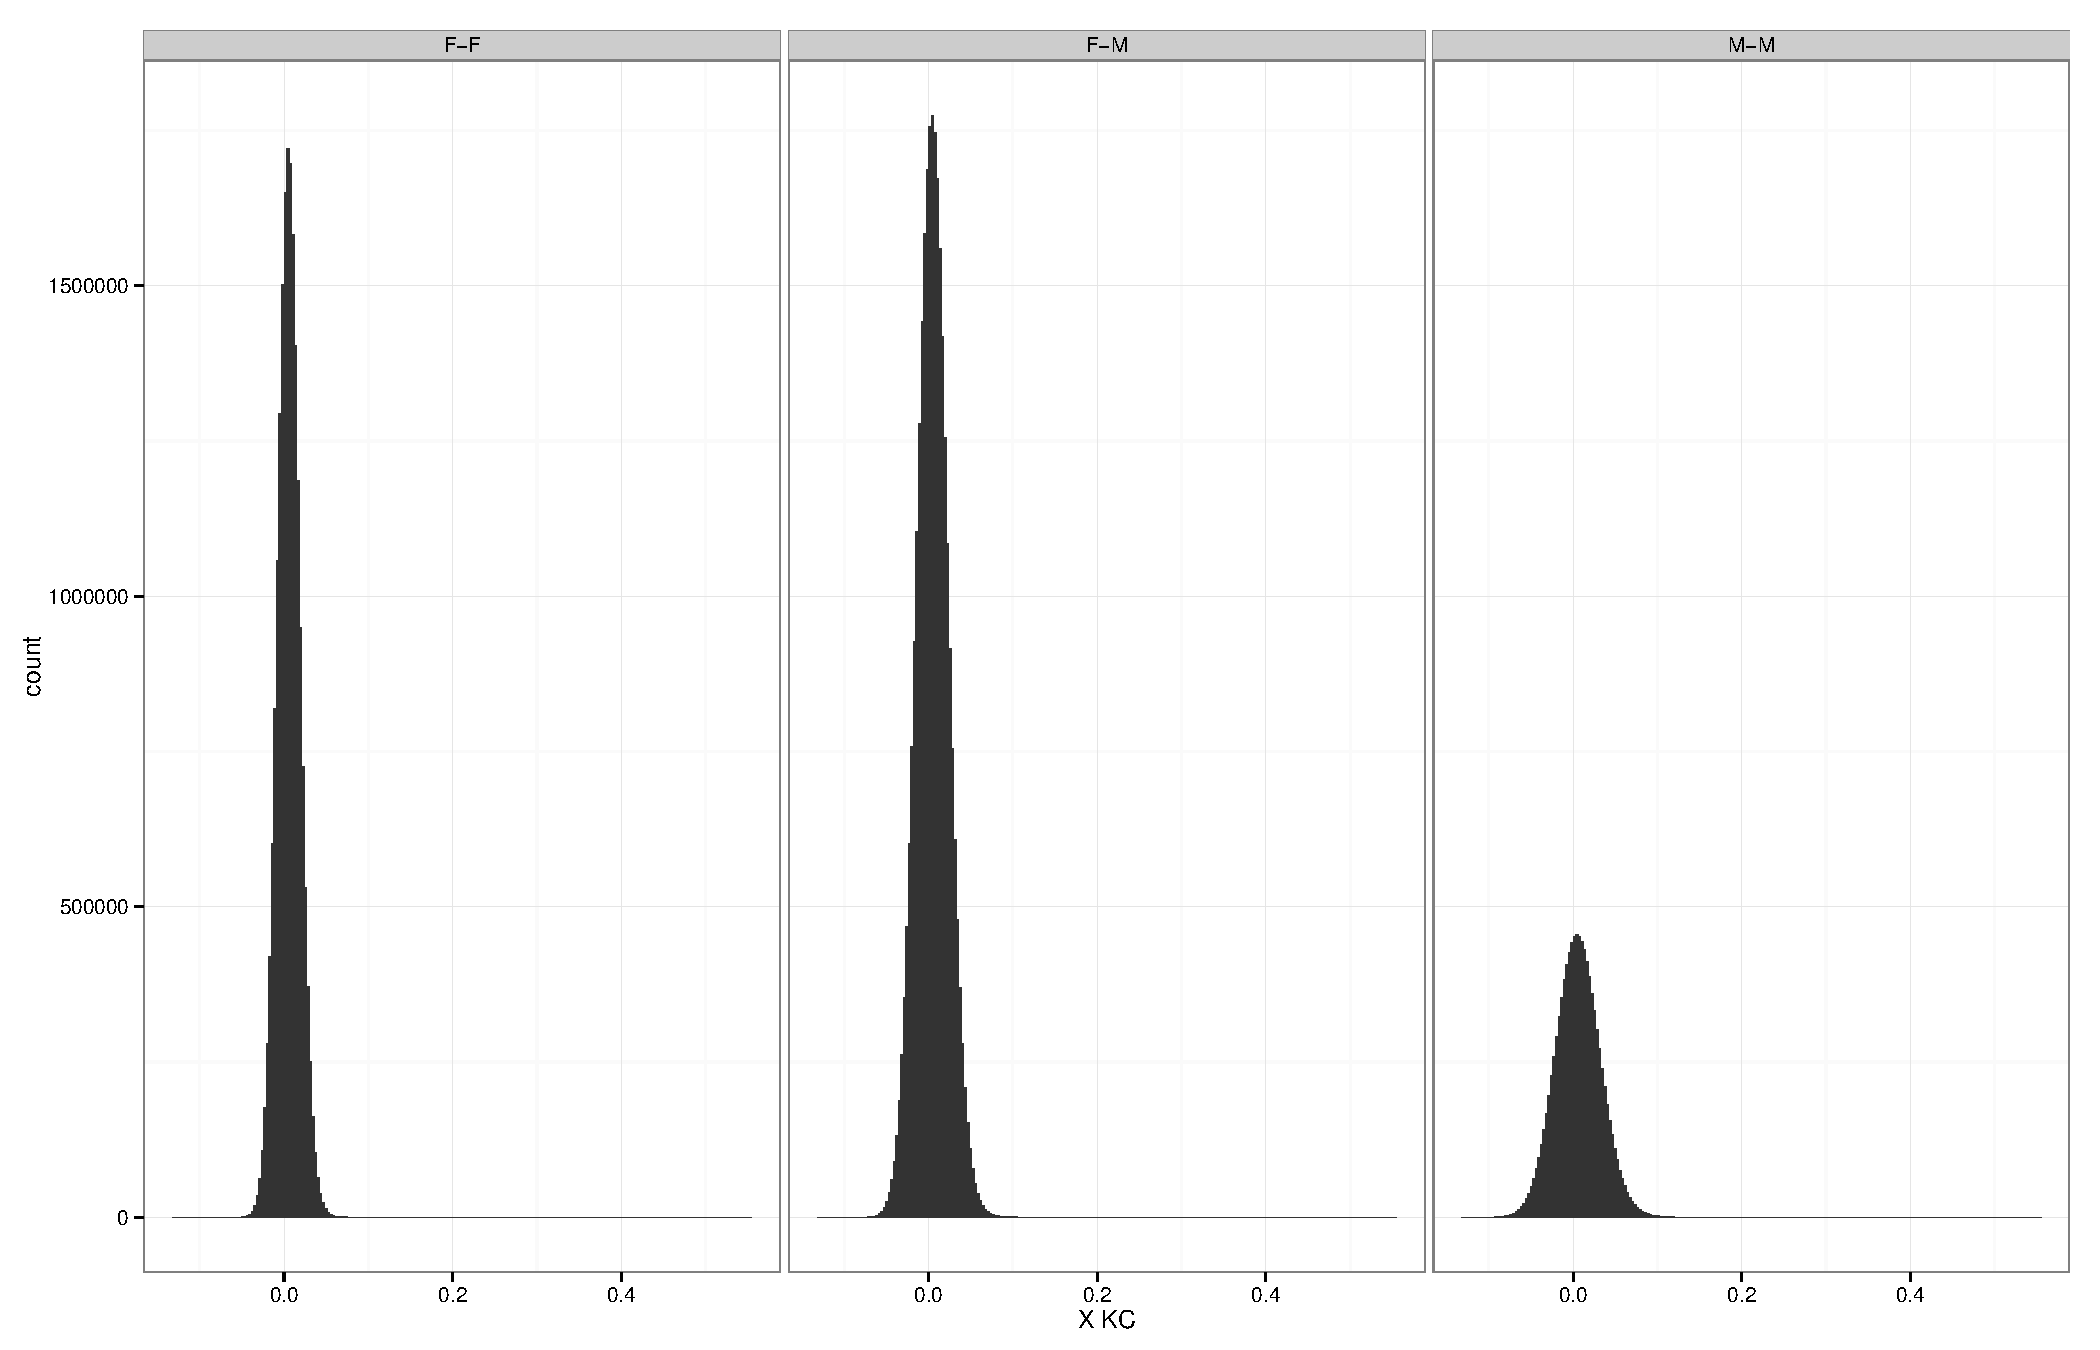
\includegraphics[height=7cm]{../olga_update_27july2015/xkc_unrel_hist_bySexPair.pdf}
\end{figure}
\end{frame}

\begin{frame}{X KC by sex, truncated}
\begin{figure}
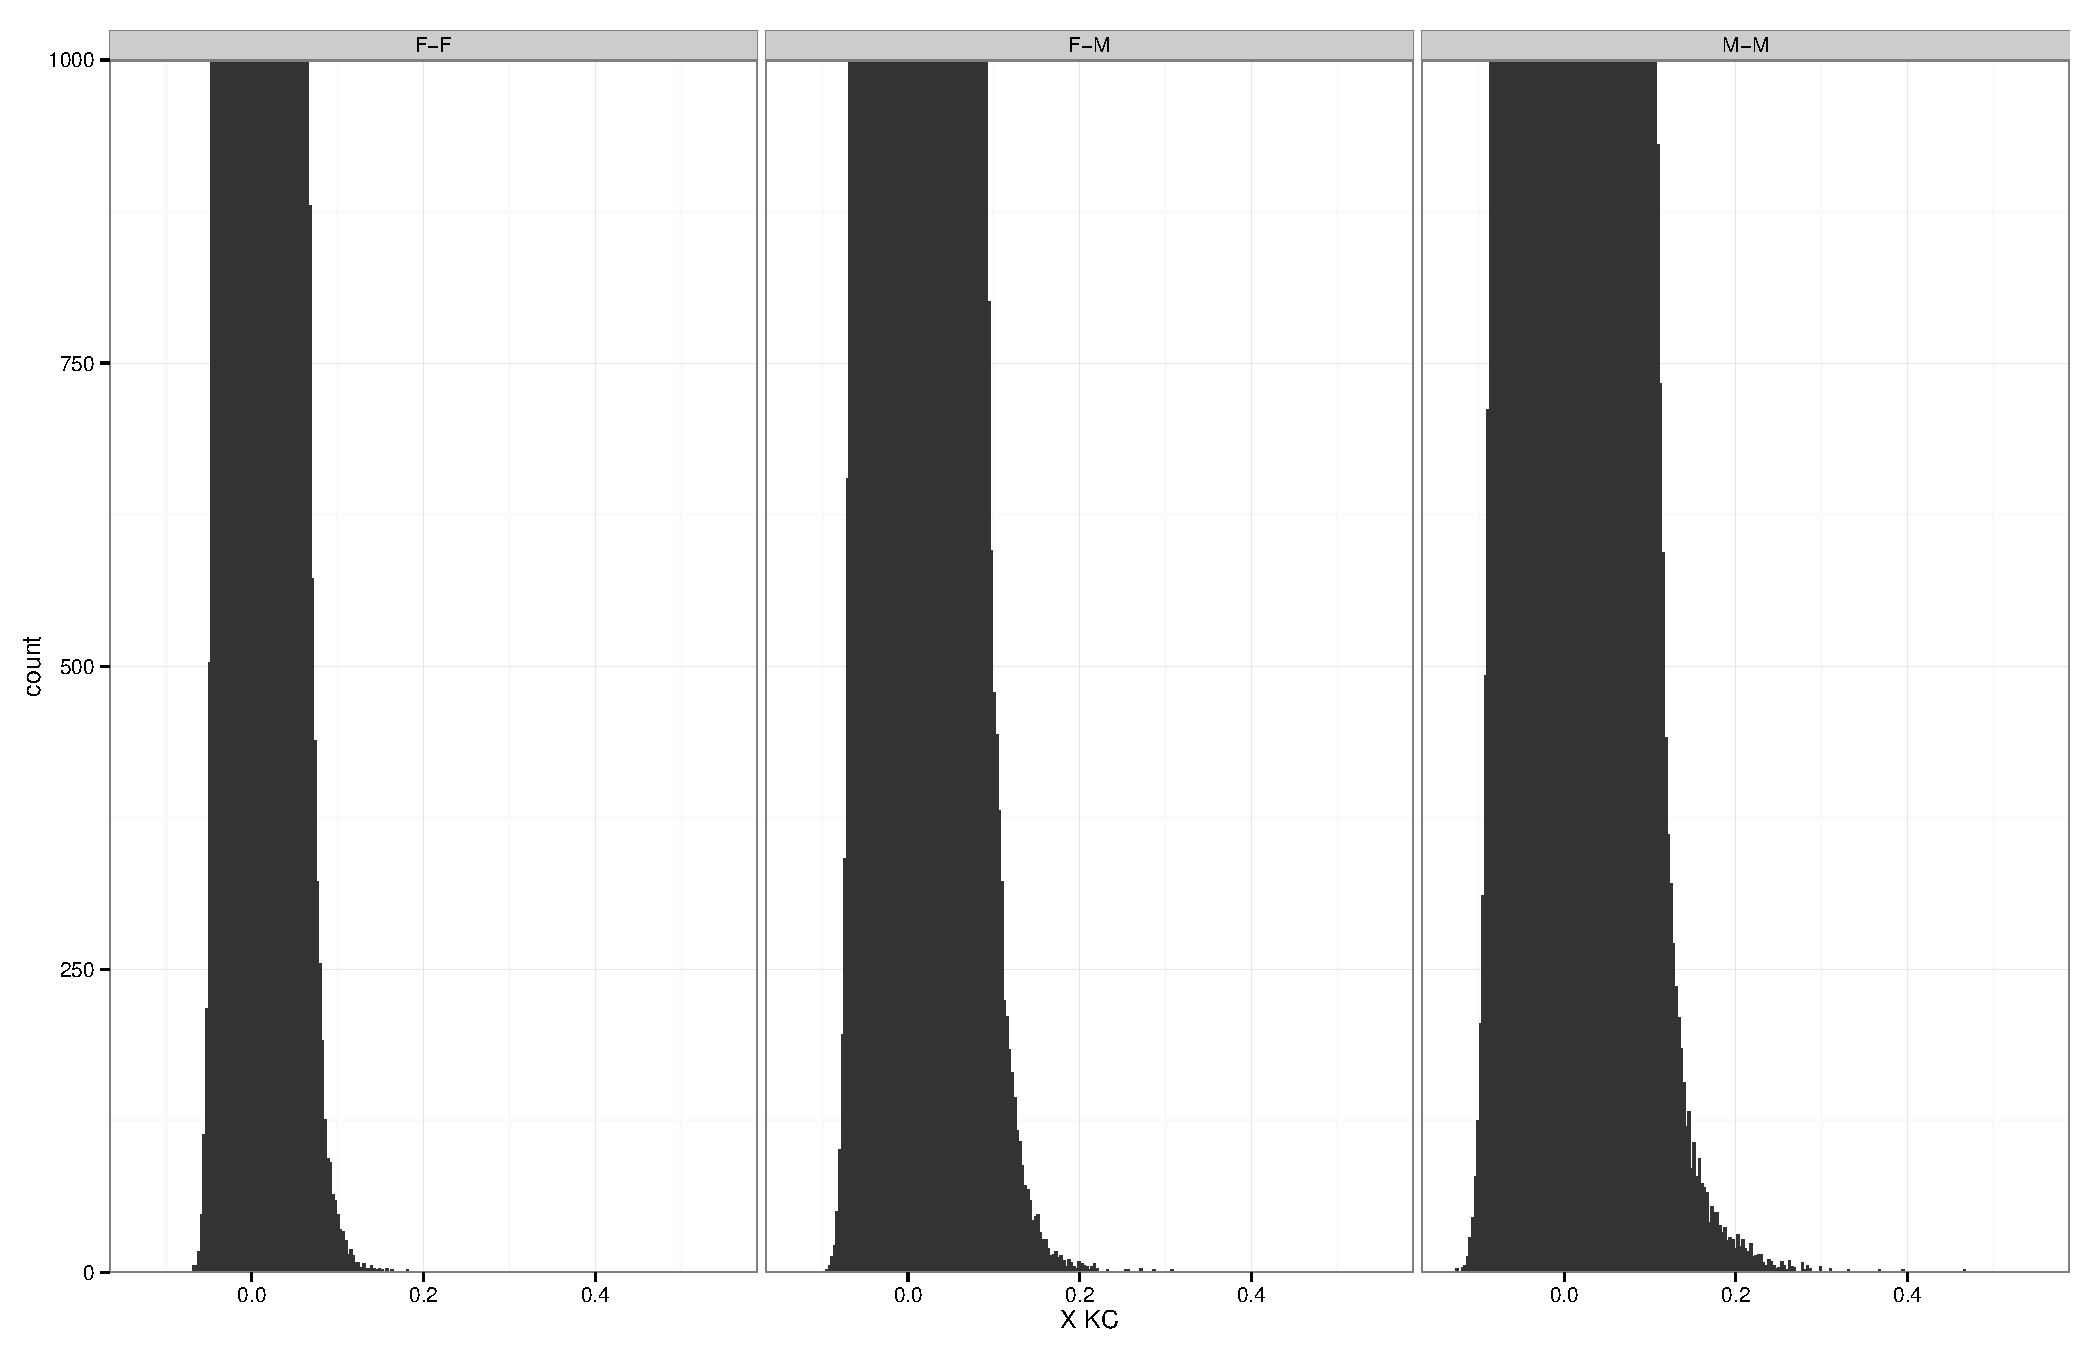
\includegraphics[height=7cm]{../olga_update_27july2015/xkc_unrel_hist_bySexPair_trunc.pdf}
\end{figure}
\end{frame}

\section[]{Estimating KC using chromosome 19}
\begin{frame}{Chr 19 KC for autosomally unrelated samples}
\begin{figure}
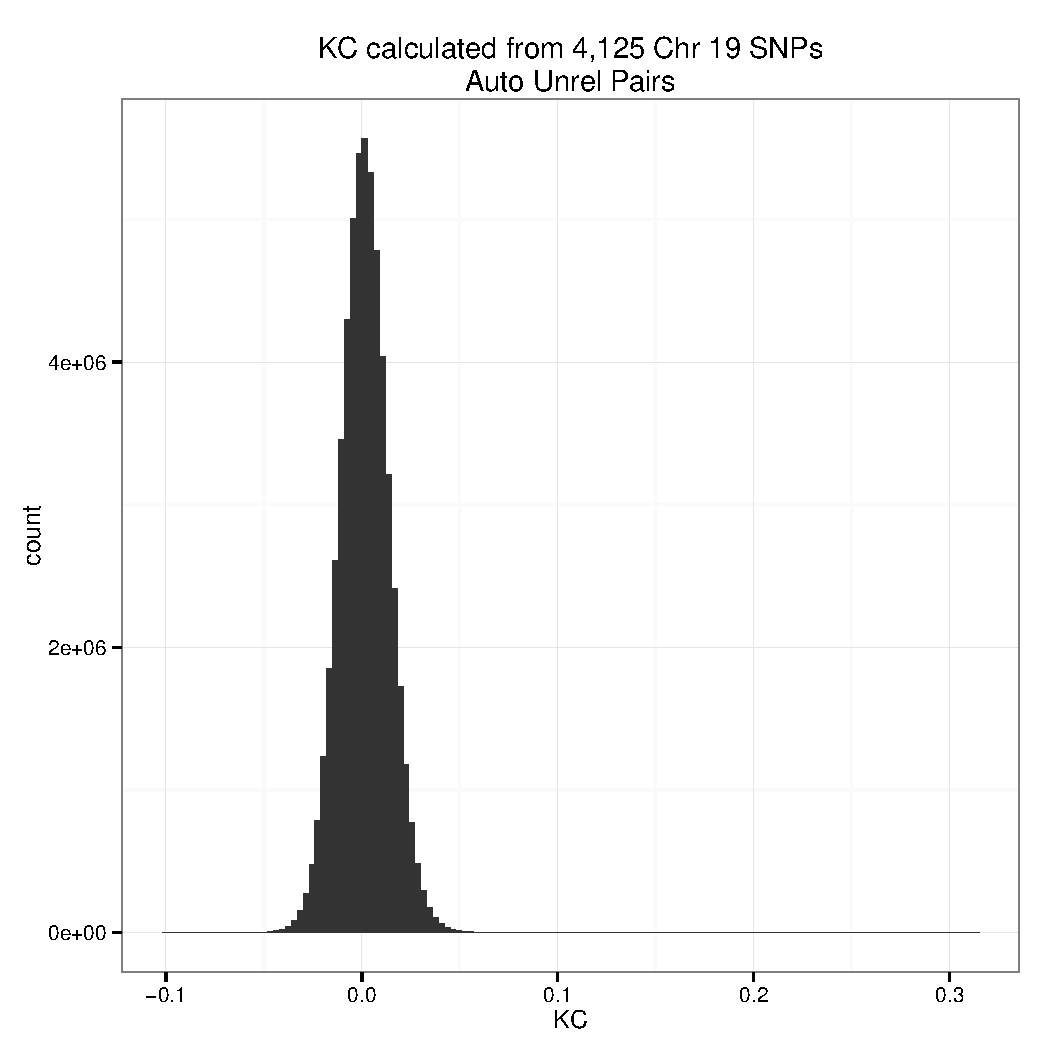
\includegraphics[height=5.9cm]{../olga_update_27july2015/kc_chr19_autounrel_hist.pdf}
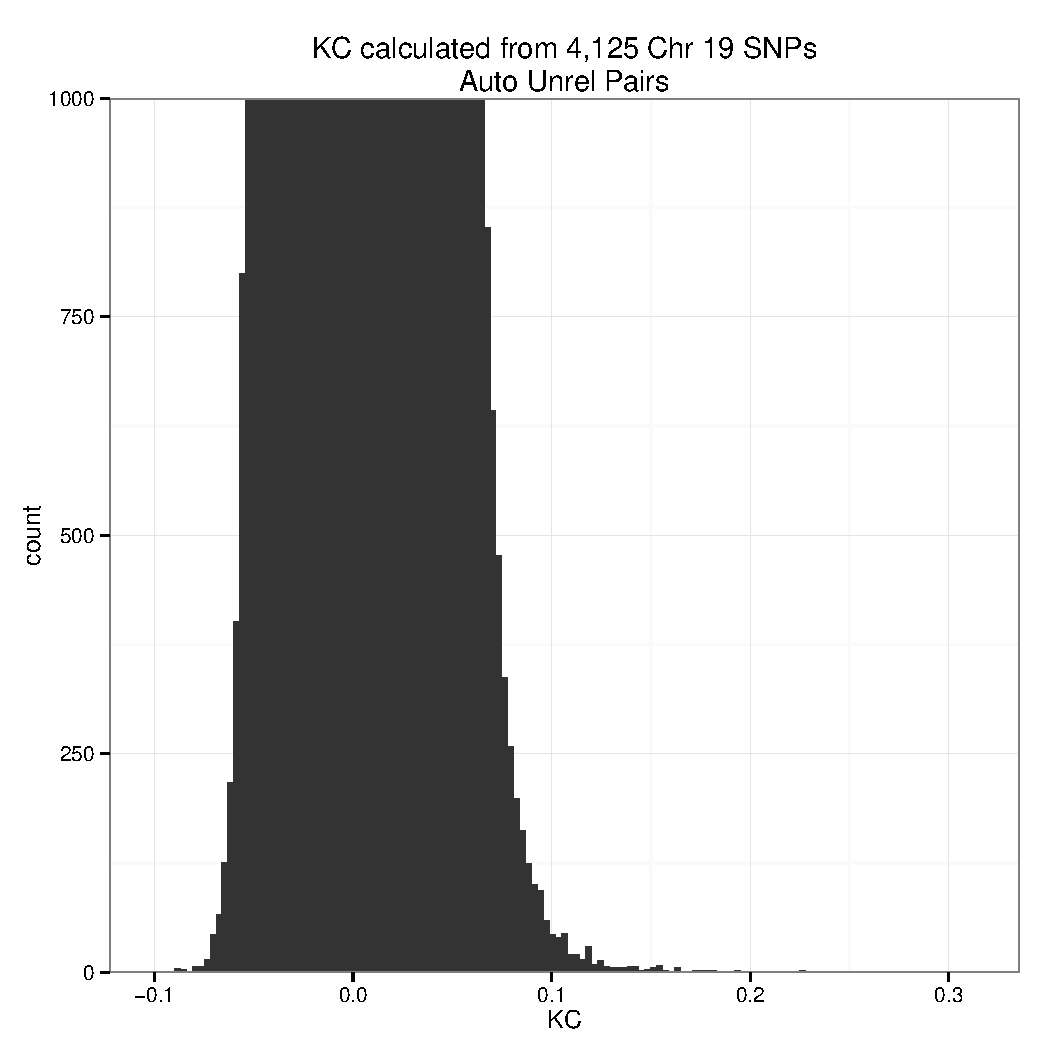
\includegraphics[height=5.9cm]{../olga_update_27july2015/kc_chr19_autounrel_hist_trunc.pdf}
\end{figure}
\end{frame}

\section[]{Comparing X and chr 19 KCs}
% chr 19 KC vs x chr FF results
\begin{frame}{Chr 19 \& X chr F-F KC for autosomally unrelated samples}
\begin{figure}
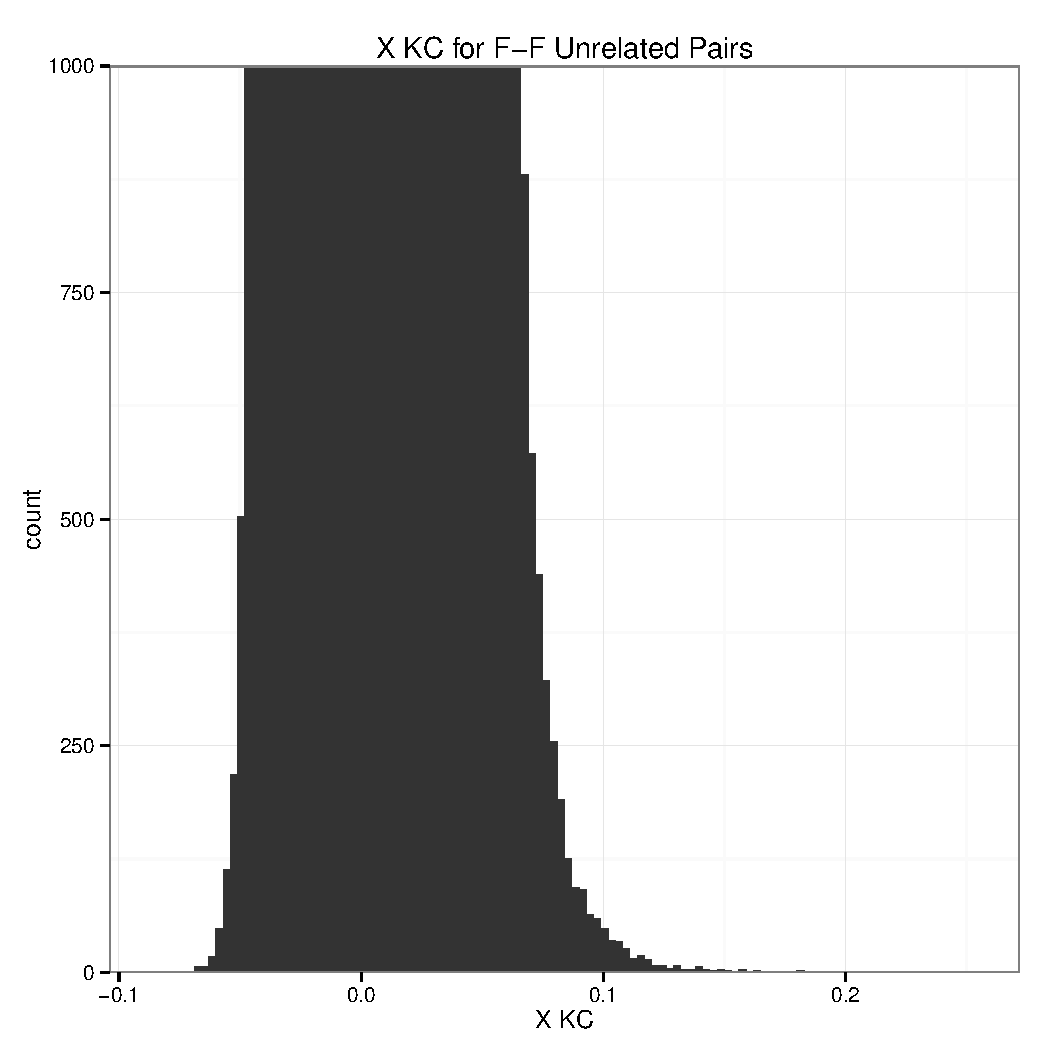
\includegraphics[height=5.9cm]{../olga_update_27july2015/xkc_unrel_hist_FFpairs_trunc.pdf}
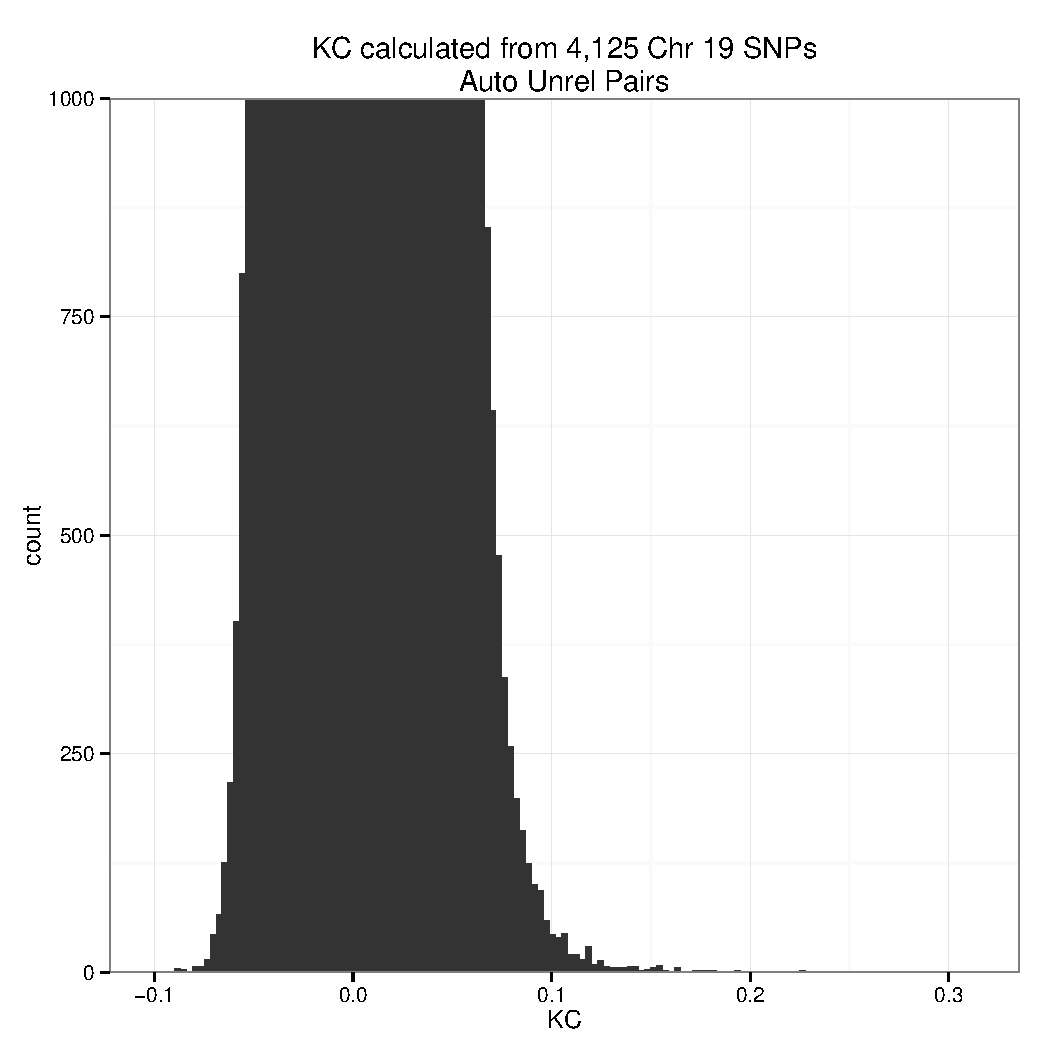
\includegraphics[height=5.9cm]{../olga_update_27july2015/kc_chr19_autounrel_hist_trunc.pdf}
\end{figure}
\end{frame}

\section[]{X chromosome SNP density}
\begin{frame}{X chromosome SNP density}
For running Beagle IBD on the X.
\begin{figure}
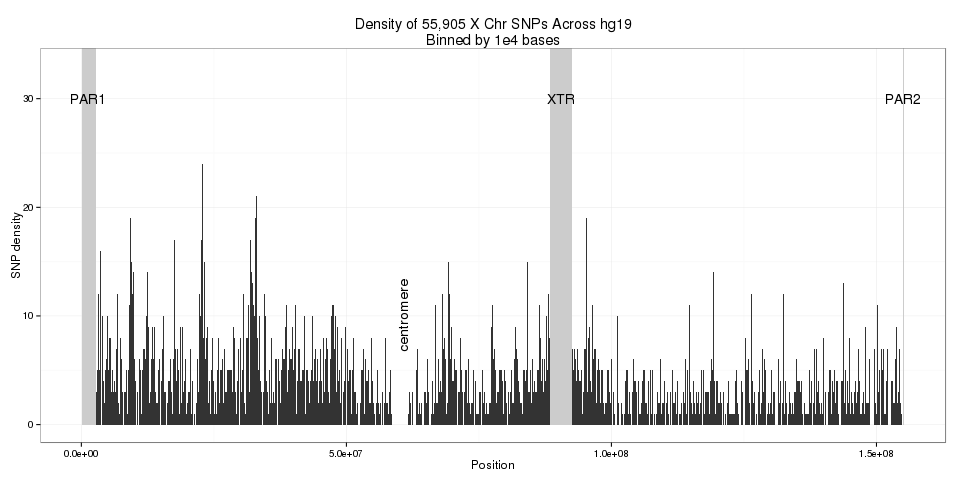
\includegraphics[width=11cm]{../olga_update_27july2015/chrX_density.png}
\end{figure}
\end{frame}

\begin{frame}{Chromosome 19 SNP density}
For comparison to the X.
\begin{figure}
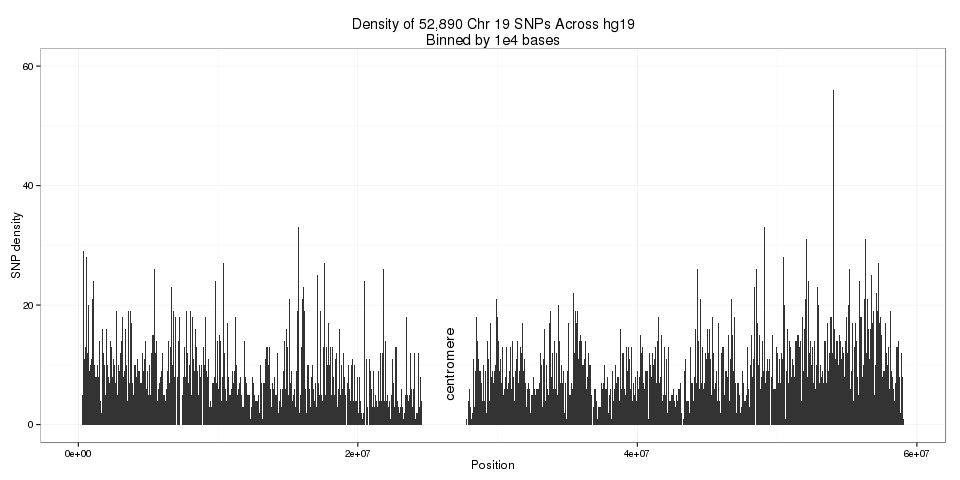
\includegraphics[width=11cm]{../olga_update_27july2015/chr19_density.png}
\end{figure}
\end{frame}

\end{document}


